\documentclass{scrreprt}

\usepackage[english,czech]{babel}
\usepackage[utf8]{inputenc}
\usepackage{graphicx}

\begin{document}

\setcounter{chapter}{6}
\chapter{Koncept jazyka na bázi virtuálniho stroje, JVM memory management, datové struktury, výjimky, objektové programování, vlákna a synchronizace. (A4B77ASS)}

\section{Typy programovacích jazyků}
Z hlediska vykonávání zdrojového kódu lze programovací jazyky dělit do dvou kategorií.
\begin{itemize}
\item \textbf{Interpretované} - přímo zdrojový kód (skript či překompilovaný byte-code) je interpretován virtuálním strojem, který běží na cílovém zařízení
\item \textbf{Kompilované} - zdrojový kód je nutné zkompilovat do strojového kódu cílového zařízení a poté lze program spustit přímo
\end{itemize}

\paragraph*{Vlastnosti interpretovaných jazyků:}
\begin{itemize}
\item[$\oplus$] nezávislost na platformě - architektura (RISC/CISC), operační systém
\item[$\oplus$] reflexe - sledování a modifikace kódu za běhu
\item[$\oplus$] dynamické typování
\item[$\oplus$] malá velikost zdrojových souborů
\item[$\ominus$] pomalejší vykonávání kódu v interpretovaném módu
\end{itemize}

\section{Java Virtual Machine (JVM)}
Je zásobníkově orientovaný virtuální stroj Javy, který interpretuje Java byte-code. Zdrojové kódy (\texttt{.java}) je proto nutné zkompilovat do byte-code (\texttt{.class}), při kompilaci nedochází k žádným optimalizacím kódu. Před spuštěním je byte-code verifikován (skoky jsou pouze na validní umístění, správná inicializace dat, type-safe reference, kontrola private a protected přístupů). Při běhu se používá JIT.

\paragraph*{Zásobníkový způsob předávání parametrů:} $(2 + 3) \times 11 + 1$
\begin{center}
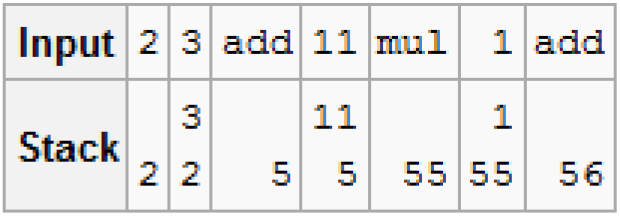
\includegraphics[scale=0.5]{img/jvm_stack}
\end{center}

\subsection{Just-in-time compiler (JIT)}
Za běhu konvertuje byte-code na nativní strojový kód. Existují různé verze pro serverové a klientské aplikace (různý stupeň optimalizace). Některé prováděné optimalizace: inlining of functions, loop unrolling, dead code elimination, loop invariant hoisting, common subexpression elimination, constant propagation, optimize branches.

\section{JVM memory management}
V JVM je použita automatická správa paměti pomocí \textbf{Garbage Collectoru (GC)} - živé (dosažitelné) objekty jsou ponechány v paměti a mrtvé (nedosažitelné) jsou smazány. Halda (\textbf{Heap}) je oblast pro dynamickou alokaci paměti pro všechny objekty a je rozdělena do secí, tzv. generací - Young a Old.

\paragraph*{Generační koncept}
Objekty jsou v haldě rozděleny do generací podle svého stáří, zpočátku jsou alokovány v Young generaci, pokud přežijí několik cyklů GC jsou povýšeny (Tenuring) do Old generace. Koncept je postaven na hypotéze, že většina objektů je krátko-žijících, tj. nedostanou se do Old generace.
\begin{center}
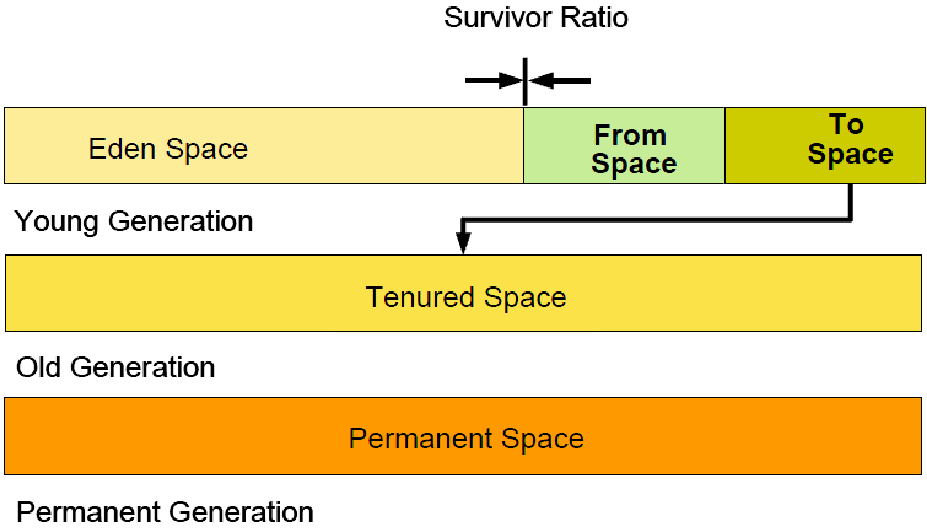
\includegraphics[scale=0.5]{img/jvm_generations}
\end{center}
\begin{description}
\item[Young] malá velikost, časté a rychlé cykly GC
\item[Old] velká velikost, málo časté a pomalé cykly GC
\item[Eden] místo pro alokaci nových objektů
\item[From/To] místo kam jsou zkopírovány přeživší objekty po běhu GC
\item[Permanent] je mimo haldu, obsahuje data pro JVM jako definice tříd, metod a další
\end{description}

\subsection{Druhy Garbage Collectorů}
\begin{itemize}
\item \textbf{Sériový collector} - používá algoritmus \emph{mark-sweep-compact} způsobem \emph{stop-the-world}, výchozí pro klientské aplikace, efektivní na 64MB haldě
\begin{center}
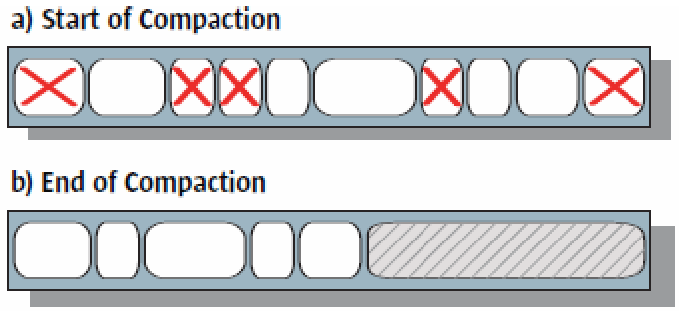
\includegraphics[scale=0.5]{img/gc_serial}
\end{center}
\item \textbf{Paralelní collector} - pro Old generaci obyčejný sériový collector, pro Young generaci navíc využívá více vláken/CPU, výchozí pro serverové aplikace a na více-jádrových systémech
\begin{center}
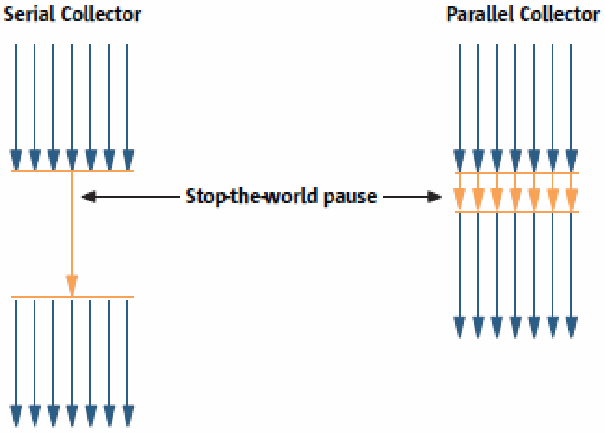
\includegraphics[scale=0.6]{img/gc_parallel}
\end{center}
\item \textbf{Souběžný (Concurrent) collector} - pro Young generaci jako paralelní collector, pro Old generaci běží souběžně s aplikací, má nízkou latenci a snižuje počet zastavení aplikace, vyžaduje ale větší haldu
\begin{center}
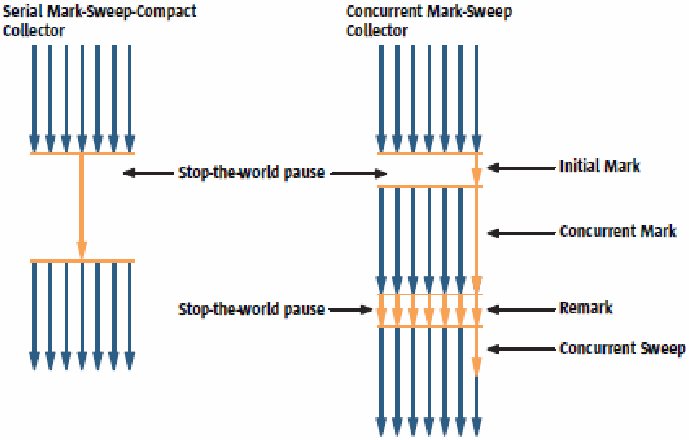
\includegraphics[scale=0.75]{img/gc_concurrent}
\end{center}
\end{itemize}

\section{Java datové struktury}
\begin{itemize}
\item \textbf{primitiva} - bez implicitní alokace, uložené na zásobníku, typy: \textsf{boolean}, \textsf{byte}, \textsf{char}, \textsf{int}, \textsf{long}, \textsf{float}, \textsf{double}
\item \textbf{objekty} - každý je potomek třídy \textsf{Object}, uloženy na haldě, existují objekty pro primitiva: \textsf{Boolean}, \textsf{Byte}, \textsf{Char}, \textsf{Integer}, \textsf{Long}, \textsf{Float}, \textsf{Double}
\item \textbf{pole (arrays)} - speciální datová struktura pro uchovávání více primitiv/objektů stejného typu v lineárním pořadí, mají definovaný limit, který je automaticky za běhu kontrolován, jsou uložené na haldě, více-dimenzionální pole = pole polí
\end{itemize}

\subsection{Autoboxing, Unboxing, Widening}
\begin{description}
\item[Autoboxing] automatická konverze primitivních datových typů na jejich objektové reprezentace
\item[Unboxing] opačný postup, objekty na primitiva
\item[Widening] automatická konverze menších primitiv na větší: \\ \textsf{byte} $\prec$ \textsf{char} $\prec$ \textsf{int} $\prec$ \textsf{long} a \textsf{float} $\prec$ \textsf{double}
\end{description}
Používání boxingu a unboxingu přináší neefektivitu. V případě více možností má widening přednost před autoboxingem. Při volání přetížených metod Java vybere tu s nejvíce specifickými typy parametrů.

\subsection{Výjimky}
Všechny extendují třídu \textsf{Throwable} (\textsf{Error}, \textsf{Exception}) a slouží k reprezentaci různých chybových stavů aplikace. Výjimky lze dělit do dvou kategorií - kontrolované (\textsf{Exception}) a nekontrolované (\textsf{Error} a \textsf{RuntimeException}). Kontrolované výjimky je nutné odchytávat pomocí \textbf{try-catch} bloku. Pro vyhození vlastní výjimky v programu souží příkaz \textbf{throw}. Výjimky také obsahují záznam obsahu zásobníku ve chvíli kdy byla tato výjimka vyhozena a případně další informace o vzniklé chybě.

\section{Vlákna a synchronizace - Java}

\subsection{Vlákna (Threads)}
Vlákna umožňují souběžné vykonávání více úkolů najednou, vytváří se buď extendováním třídy \textsf{Thread} nebo implementací rozhraní \textsf{Runnable}. Hlavní je metoda \textbf{run()} obsahující kód, který vlákno vykonává. Jeden proces může mít více vláken, která sdílí společný adresní prostor, ale všechny mají vlastní zásobník a lokální proměnné. Každé vlákno má: ID, jméno, prioritu, thread group, uncaught exception handler, deamon flag, class loader, interrupted flag, status.

\subsection{Synchronizace}
Při práci s více vlákny je často nutná jejich synchronizace a umožnění bezpečného přístupu ke sdíleným prostředkům. K tomu existuje několik technik.
\begin{itemize}
\item \textbf{Synchronized} - S každým objektem je asociován tzv. \emph{monitor}, který umožňuje synchronizaci vláken nad tímto objektem použitím bloku \textbf{synchronized}. Pro vstup do tohoto bloku je nutné aby příslušné vlákno vlastnilo tento monitor, v jednu chvíli ale může monitor vlastnit pouze jedno vlákno. Pokud není monitor pro vlákno dostupný, jeho běh je zastaven dokud se monitor neuvolní. Pro synchronizaci celé metody je možné použít klíčové slovo \textbf{synchronized}.

\item \textbf{Reentrant Locks} - Obdoba předchozí synchronizační techniky s manuálním získáváním a uvolňováním zámků - metody: \textbf{lock()}, \textbf{unlock()}, \textbf{tryLock()}. Zámky je nutné manuálně vytvářet jako objekty \textsf{ReentrantLock}, zámky je možné vytvořit \emph{fair}, tj. první čekající vlákno bude první kdo získá zámek. Používání Reentrant zámků je v praxi efektivnější než použití synchronized, ale zámky jsou běžné objekty na haldě.
\begin{verbatim}
lock.lock(); 
try {
    // do some staff ...
} finally {
    lock.unlock()
}
\end{verbatim}

\item \textbf{Volatile proměnné} - Jsou obyčejné proměnné, které ale mají zaručen atomický read/write přístup. Tyto proměnné nejsou nikdy uloženy lokálně pro jednotlivá vlákna, ale je vždy přistupováno přímo do hlavní paměti. Nevhodné pro \emph{read-update-write} operace. Použití pomocí klíčového slova \textbf{volatile}.

\item \textbf{Atomické proměnné} - Umožňují atomický read/write přístup i \emph{read-update-write} operace. Používají se speciální atomické instrukce procesoru - \textbf{CMPXCHG} (compare and exchange) nebo \textbf{CAS} (compare and swap). Pro základní datové typy existují \textsf{AtomicBoolean}, \textsf{AtomicInteger}, \textsf{AtomicLong} a \textsf{AtomicReference} s operacemi \textbf{get()}, \textbf{set()}, \textbf{compareAndSet()}, \textbf{addAndGet()}, \textbf{incrementAndGet()}, \textbf{decrementAndGet()}.

\item \textbf{Neblokující algoritmy} - Synchronizační algoritmy, které nepoužívají zámky ani čekání vláken, ale jsou postavené na atomických CAS operacích. Princip je, že se v nekonečné smyčce kontroluje stav atomické proměnné, dokud není možné bezpečně pokračovat dále. Tento princip výkonnostně převyšuje blokující algoritmy protože většina CAS operací uspěje na první pokus. Další výhodou je, že odstraňuje nadbytečné uspávání vláken a přepínání kontextu.
\end{itemize}

\section{Návrhové vzory pro objektové programování}
\begin{itemize}
\item \textbf{Immutable object} - objekt, který po dobu svého života nemění žádné své vlastnosti, all fields are final, no setters
\item \textbf{Factory method, Abstract factory} - k vytváření objektů se používají speciální metody či tovární třídy
\item \textbf{Lazy initialization} - k výpočtům, inicializacím objektů a dalších dat dochází až v případě prvního použití
\item \textbf{Singleton} - pro danou třídu existuje pouze jedna instance v rámci celé aplikace
\item \textbf{Multiton} - pro danou třídu existuje několik instancí s různými parametry v rámci celé aplikace
\item \textbf{Strategy} - definice společného rozhraní pro skupinu podobných algoritmů, umožňuje zaměňovat různé implementace
\item \textbf{Composite} - skládání objektů do stromových struktur, ke skupině objektů je přistupováno jako k jediné instanci (Nodes and Leafs)
\item \textbf{Iterator} - umožňuje sekvenční procházení kolekce po jednotlivých prvcích bez odhalení vnitřní struktury této kolekce
\item \textbf{Command} - zastřešuje veškeré informace potřebné pro volání metod později - client, invoker, receiver
\end{itemize}

\end{document}
